\documentclass{article}
\usepackage[utf8]{inputenc}
\usepackage{amsmath}
\usepackage{graphicx}
\usepackage{amssymb}

\title{ASSIGNMENT_1}
\author{AI21BTECH11021}
\date{March 2022}

\begin{document}

\maketitle

\section*{Question 3 (c)}
\begin{figure}[h!]
    \centering
    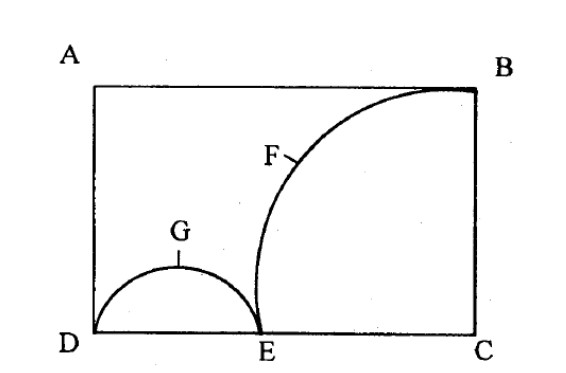
\includegraphics[scale = 0.5]{Figure_1.jpg}
    \caption{rectangle}
    \label{fig:my_label}
\end{figure}

In the figure given below, \textbf{ABCD} is a rectangle.\textbf{AB} = 14 cm\textbf{BC} = 7 cm.\\
From the rectangle, a quarter circle \textbf{BFEC} and a semicircle \textbf{DGE} are removed.\\
Calculate the area of the remaining piece of the rectangle.\\
( Take $ \pi = 22/7 $)\\

\section*{solution:}
\begin{center}
    $Area of rectangle = length*width$\\
    
    $Area of circle =\pi*radius^2 $\\
\end{center}
 \begin{center}
     so area of rectangle $ABCD = 14cm*7cm = 98cm^2$.\\
 \end{center}

Area of BFEC region is $\frac{1}{4}*\pi*(7cm)^2 = \frac{77}{2}cm^2 $ here radius is BC.\\

Area of GDE region is $\frac{1}{2}*\pi*(\frac{7}{2}cm)^2= \frac{77}{4}cm^2$ the length\\ 
of $BC = EC = 7cm$ also length of $AB = DC = 14cm$ so $DE = DC - EC = 7cm$ therefore\\
the radius of semicircle $GDE = \frac{DE}{2} = \frac{7}{2}cm$\\

Area of remaining piece of rectangle ADGEFBA = area of rectangle - area of semicircle - are of quarter circle.\\
$$\implies area required =98cm^{2} - \frac{77}{2}cm^{2} - \frac{77}{4}cm^{2} = \frac{161}{4}cm^{2} = 40.25cm^{2} $$ \\
\begin{center}
 \therefore Area  of the region $ ADGEFB = 40.25cm^2$    
\end{center}

\begin{figure}[h!]
    \centering
    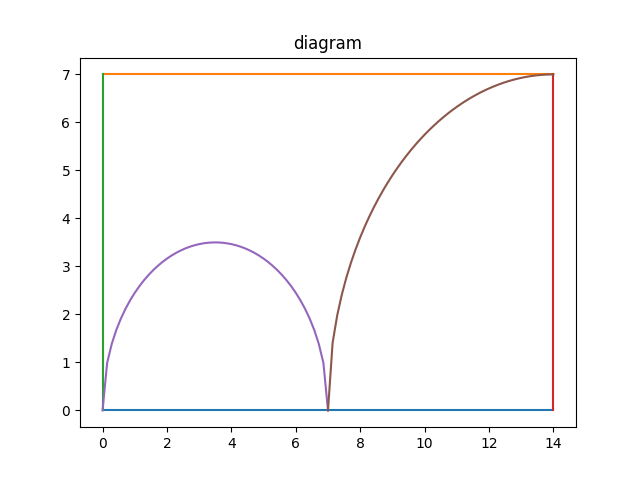
\includegraphics[scale = 0.5]{Figure_2.png}
    \caption{python programmed}
    \label{fig:my_label}
\end{figure}
\begin{center}
Verifying the calculation in python gives    
\end{center}

\begin{figure}[h!]
    \centering
    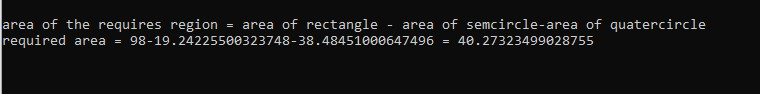
\includegraphics[scale = 0.6]{Figure_3.jpg}
    \caption{python}
    \label{fig:my_label}
\end{figure}

\end{document}
